% Companion for the separate initialization ablation (subsection 5.5).
\subsection{Robustness to parameter initialization}
\label{subsec:experimental_initialization_statistics}
The initialization ablation varies the starting point over 30 independently
drawn initializations while retaining a fixed input/noise record within
each implementation. Final errors were compared using the outcome and
tests in Section~\ref{subsec:experimental_hypothesis_tests}, with separate
Holm families for this study. Paired tests use the shared starting point
and data record of each original experiment. When a method fails to return
a valid estimate, its output cannot define a parameter-error difference;
accuracy tests therefore condition on jointly valid pairs and failed
outputs are not awarded as wins to their competitors. All finite extreme
outcomes were retained, including those suppressed only in boxplot displays.

Tables~\ref{tab:expstats_summary_initialization}--
\ref{tab:expstats_advantages_initialization} and
Figures~\ref{fig:expstats_wins_example_1_initialization_fsm}--
\ref{fig:expstats_wins_example_cstr_initialization_pl} show strong
initialization-dependent differences. BI-HMC provides valid point estimates
for all 30 initializations and has significantly favorable errors against
all eight available comparators in each reported case. The PL BI-HMC
contrasts require particular qualification: the reused Python reference
and the MATLAB methods use different fixed data records and different
starting-point draws. Their rank-sum results compare these conditional
error distributions; they do not isolate the effect of initialization
or establish a causal robustness advantage under identical observed data.
The FSM paired contrasts provide the directly controlled comparison.

Among the optimization rules, LHAM-3-TIK is favorable in Example~1/PL,
with significant advantages over six comparators and 30 valid outcomes;
its comparison with LHAM-1-TIK is inconclusive. This behavior does not
transfer uniformly to CSTR/PL, where RLS, WS-GNI, GHAM-1-dH, and
GHAM-2-dH attain significantly lower errors than both LHAM variants on
jointly valid starts. In the two PL cases, however, RLS and WS-GNI return
only 14 and 16 finite estimates, respectively, whereas both LHAM variants
return 30. Consequently, conditional accuracy and successful completion
must be considered separately. For Example~1/FSM, GHAM-2-H and GHAM-2-I
frequently produce smaller errors than the LHAM rules, but GHAM-2-I has
only 18 valid outcomes and GHAM-2-H includes a rare, very large finite
error. A sign-test advantage alone does not imply smaller tail risk.
For CSTR/FSM, both LHAM variants significantly outperform all evaluated
GHAM rules but neither significantly outperforms Newton or GI.
The initialization study therefore supports case-specific trade-offs
between conditional accuracy and completion frequency, rather than a
single optimizer that is uniformly robust to initialization.

\begin{table}[!htbp]
\centering
\small
\caption{Significant pairwise differences after Holm correction: initialization ablation.}
\label{tab:expstats_summary_initialization}
\setlength{\tabcolsep}{5pt}
\renewcommand{\arraystretch}{1.12}
\begin{tabular}{@{}lccc@{}}
\toprule
Case & Family size & Paired sign & Rank-sum \\
\midrule
Example 1/FSM & 36 & 26/36 & -- \\
Example 1/PL & 36 & 14/28 & 8/8 \\
CSTR/FSM & 36 & 30/36 & -- \\
CSTR/PL & 36 & 24/28 & 8/8 \\
\bottomrule
\end{tabular}
\par\smallskip
\begin{minipage}{\linewidth}\footnotesize
The paired accuracy tests condition on jointly valid outcomes. Independent RS tests involving the reused BI-HMC reference compare separate starting-point samples on different fixed records; they do not isolate initialization robustness under identical observed data.
\end{minipage}
\end{table}
\begin{table}[!htbp]
\centering
\small
\caption{Valid final estimates among 30 attempted initializations.}
\label{tab:expstats_initialization_valid}
\setlength{\tabcolsep}{5pt}
\renewcommand{\arraystretch}{1.12}
\begin{tabular}{@{}lcccc@{}}
\toprule
Method & Ex. 1/FSM & Ex. 1/PL & CSTR/FSM & CSTR/PL \\
\midrule
BI-HMC & 30 & 30 & 30 & 30 \\
RLS & -- & 14 & -- & 14 \\
Newton / WS-GNI & 30 & 16 & 30 & 16 \\
GI / WS-GGI & 24 & 30 & 30 & 30 \\
GHAM-1-dH & 30 & 29 & 30 & 30 \\
GHAM-2-dH & 28 & 26 & 30 & 28 \\
GHAM-2-H & 30 & -- & 30 & -- \\
GHAM-2-I & 18 & 28 & 30 & 28 \\
LHAM-1-TIK & 30 & 30 & 30 & 30 \\
LHAM-3-TIK & 30 & 30 & 30 & 30 \\
\bottomrule
\end{tabular}
\par\smallskip
\begin{minipage}{\linewidth}\footnotesize
A dash denotes an unavailable method. Finite estimates are not necessarily converged; the saved valid-output policy also includes finite stalled or iteration-limited estimates and valid Bayesian point estimates with sampler warnings. No success-rate hypothesis is inferred from the accuracy tests.
\end{minipage}
\end{table}
\begin{table}[!htbp]
\centering
\small
\caption{Significant advantages:disadvantages for each method in the initialization comparisons.}
\label{tab:expstats_advantages_initialization}
\setlength{\tabcolsep}{5pt}
\renewcommand{\arraystretch}{1.12}
\begin{tabular}{@{}lcccc@{}}
\toprule
Method & Ex. 1/FSM & Ex. 1/PL & CSTR/FSM & CSTR/PL \\
\midrule
BI-HMC & 8:0 & 8:0 & 8:0 & 8:0 \\
RLS & -- & 1:2 & -- & 5:1 \\
Newton / WS-GNI & 3:4 & 1:2 & 4:1 & 4:1 \\
GI / WS-GGI & 0:5 & 0:7 & 4:1 & 1:7 \\
GHAM-1-dH & 4:3 & 2:2 & 3:5 & 4:3 \\
GHAM-2-dH & 0:1 & 2:2 & 0:8 & 5:1 \\
GHAM-2-H & 5:1 & -- & 1:6 & -- \\
GHAM-2-I & 5:1 & 0:5 & 1:6 & 0:8 \\
LHAM-1-TIK & 1:5 & 2:1 & 5:1 & 2:6 \\
LHAM-3-TIK & 0:6 & 6:1 & 4:2 & 3:5 \\
\bottomrule
\end{tabular}
\par\smallskip
\begin{minipage}{\linewidth}\footnotesize
Each entry counts significantly better:worse outcomes against other methods, using Holm-adjusted $p<0.05$. These counts summarize pairwise conclusions; they are not a pooled significance test or a total ranking. A dash means there are no testable comparisons for that method.
\end{minipage}
\end{table}
\begin{figure}[p]
\centering
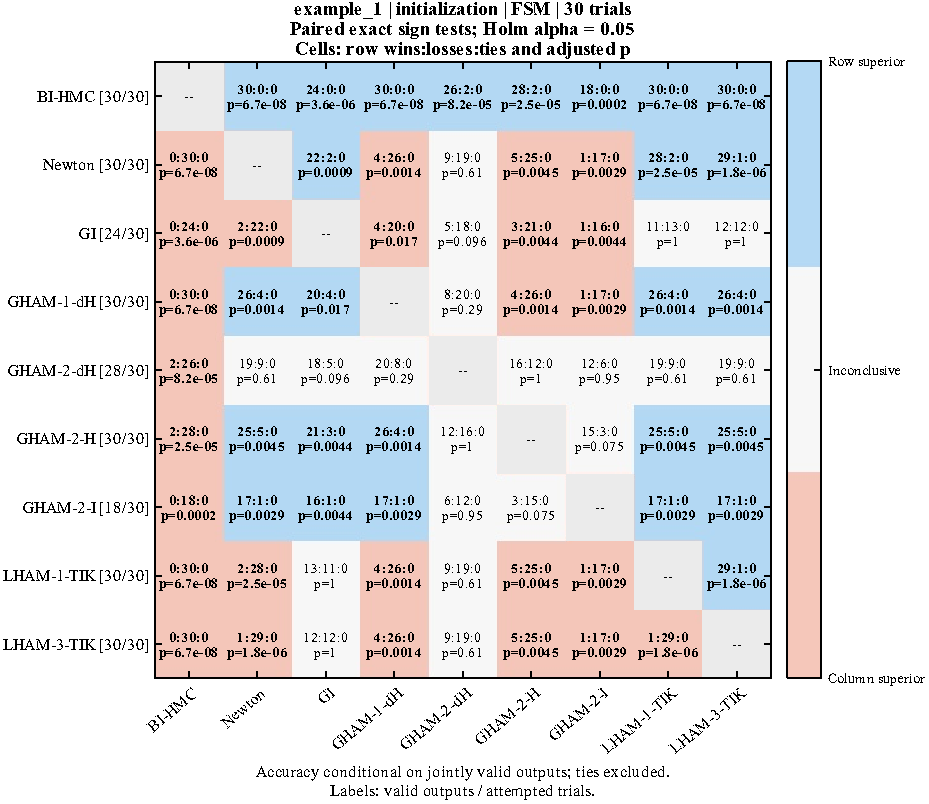
\includegraphics[width=\linewidth,height=.77\textheight,keepaspectratio]{output/experimental_statistics/parameter_error_wins_example_1_initialization_fsm.pdf}
\caption{Final-parameter-error comparison matrix for Example 1/FSM, 30 randomized initializations. Blue cells favor the row method and red cells favor the column method after Holm correction ($\alpha=0.05$); white cells are inconclusive. Paired cells show row wins:losses:ties and $p_{\rm H}$. Cells marked RS use independent rank-sum tests and show $\widehat A_{\rm row,col}$ and $p_{\rm H}$. Grey diagonal or NA entries are not tests.}
\label{fig:expstats_wins_example_1_initialization_fsm}
\end{figure}
\begin{figure}[p]
\centering
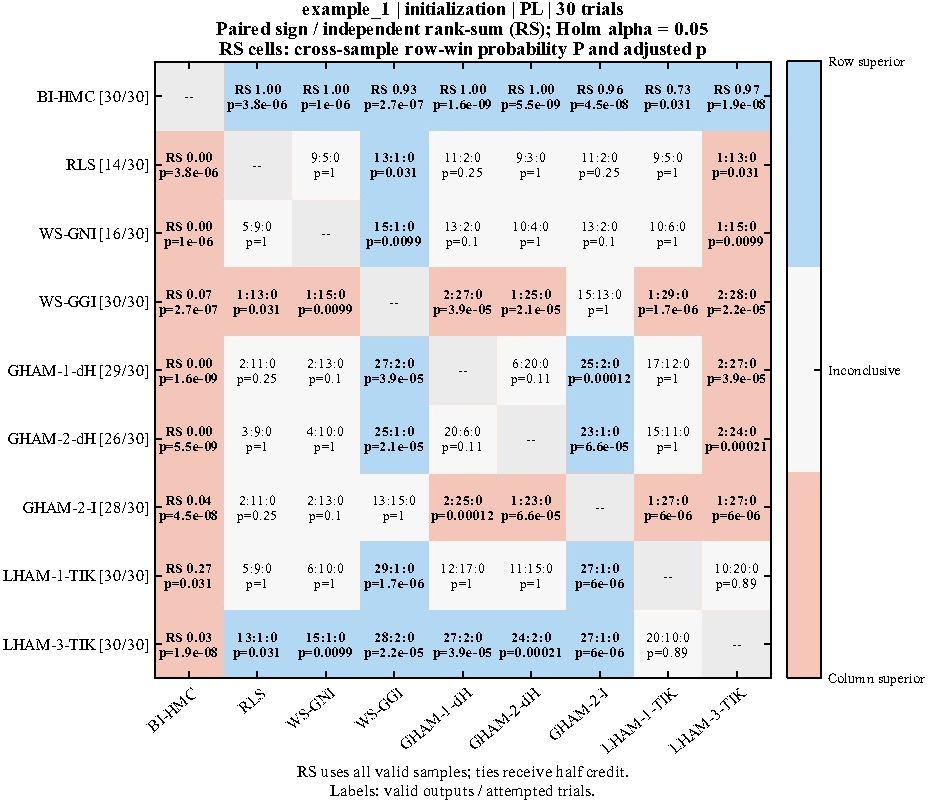
\includegraphics[width=\linewidth,height=.77\textheight,keepaspectratio]{output/experimental_statistics/parameter_error_wins_example_1_initialization_pl.pdf}
\caption{Final-parameter-error comparison matrix for Example 1/PL, 30 randomized initializations. Blue cells favor the row method and red cells favor the column method after Holm correction ($\alpha=0.05$); white cells are inconclusive. Paired cells show row wins:losses:ties and $p_{\rm H}$. Cells marked RS use independent rank-sum tests and show $\widehat A_{\rm row,col}$ and $p_{\rm H}$. Grey diagonal or NA entries are not tests.}
\label{fig:expstats_wins_example_1_initialization_pl}
\end{figure}
\begin{figure}[p]
\centering
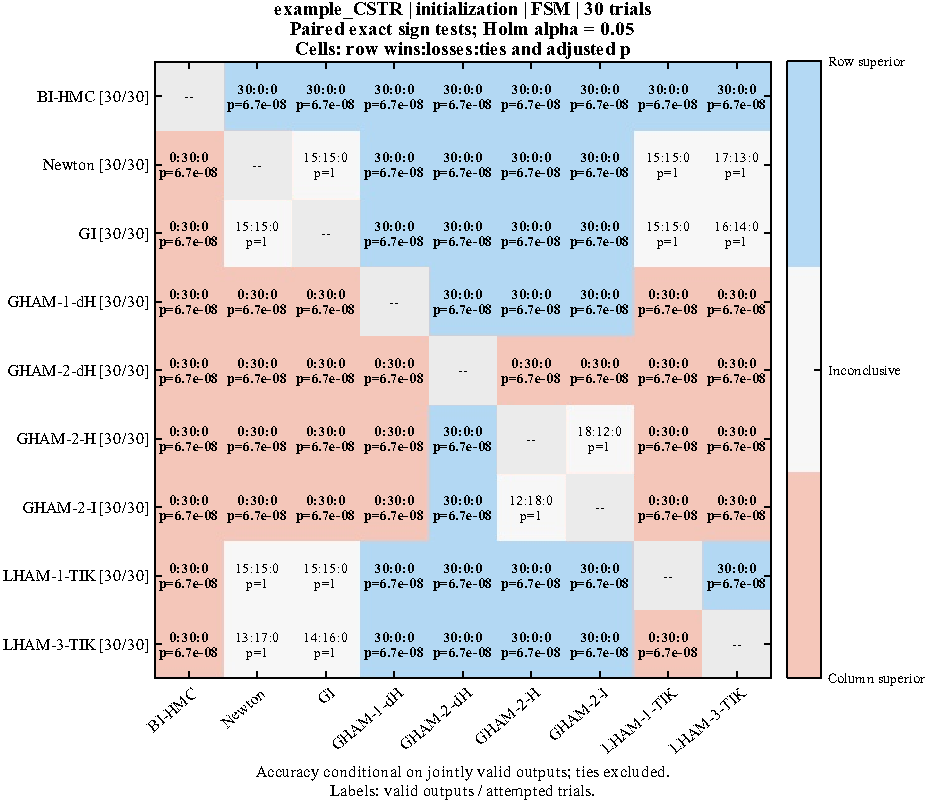
\includegraphics[width=\linewidth,height=.77\textheight,keepaspectratio]{output/experimental_statistics/parameter_error_wins_example_cstr_initialization_fsm.pdf}
\caption{Final-parameter-error comparison matrix for CSTR/FSM, 30 randomized initializations. Blue cells favor the row method and red cells favor the column method after Holm correction ($\alpha=0.05$); white cells are inconclusive. Paired cells show row wins:losses:ties and $p_{\rm H}$. Cells marked RS use independent rank-sum tests and show $\widehat A_{\rm row,col}$ and $p_{\rm H}$. Grey diagonal or NA entries are not tests.}
\label{fig:expstats_wins_example_cstr_initialization_fsm}
\end{figure}
\begin{figure}[p]
\centering
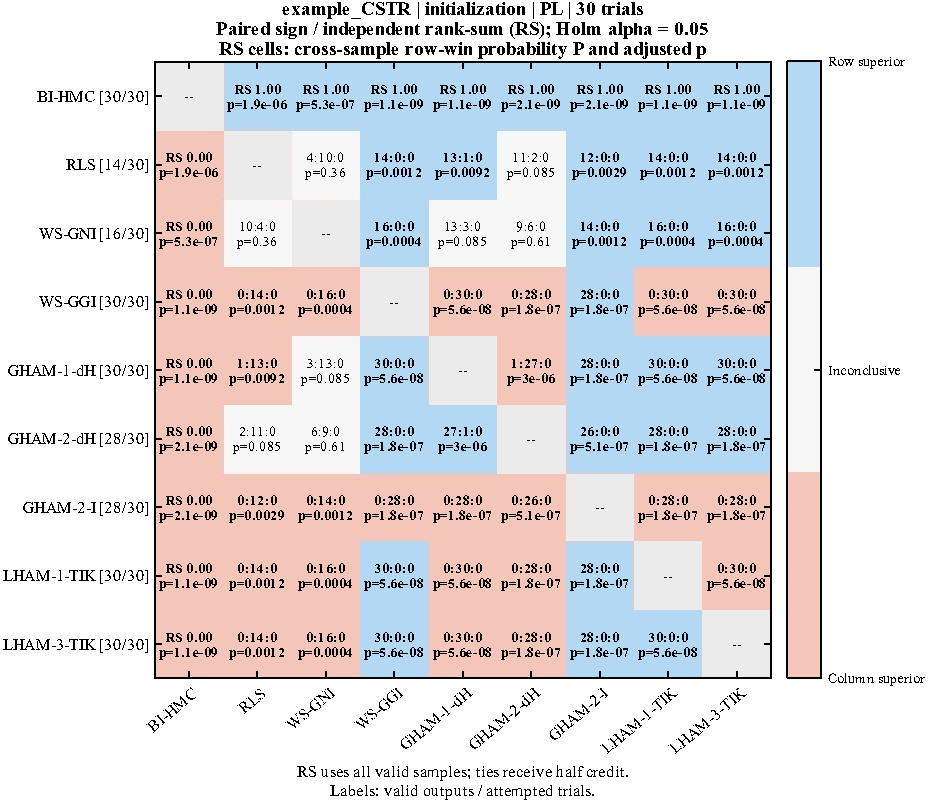
\includegraphics[width=\linewidth,height=.77\textheight,keepaspectratio]{output/experimental_statistics/parameter_error_wins_example_cstr_initialization_pl.pdf}
\caption{Final-parameter-error comparison matrix for CSTR/PL, 30 randomized initializations. Blue cells favor the row method and red cells favor the column method after Holm correction ($\alpha=0.05$); white cells are inconclusive. Paired cells show row wins:losses:ties and $p_{\rm H}$. Cells marked RS use independent rank-sum tests and show $\widehat A_{\rm row,col}$ and $p_{\rm H}$. Grey diagonal or NA entries are not tests.}
\label{fig:expstats_wins_example_cstr_initialization_pl}
\end{figure}
